\tikzstyle{org} = [rectangle, draw, font=\footnotesize,
                   fill=gray!30, minimum width=18em, text width=18em]

\tikzstyle{ext} = [rectangle, draw, rounded corners,
                   text centered, text width=5em]

\tikzstyle{proc} = [->, thick, bend right, bend angle=22.5]
\tikzstyle{data} = [->, thick, bend angle=90, bend right, distance=4em]
\tikzstyle{data-label} = [left, midway, text width=4em, text centered]
\tikzstyle{ref-label} = [right, midway, text width=4em, text centered]

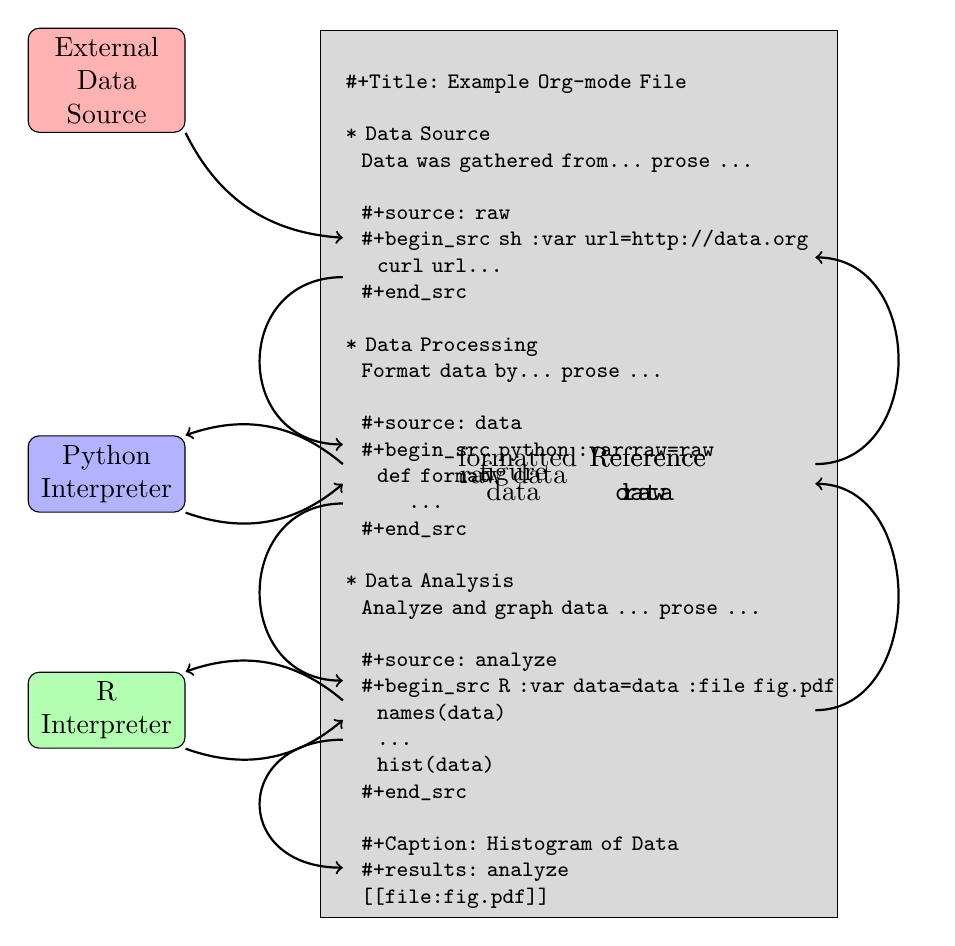
\begin{tikzpicture}
  \node [org] at (0,0) {
\begin{verbatim}
  #+Title: Example Org-mode File
  
  * Data Source
    Data was gathered from... prose ...

    #+source: raw
    #+begin_src sh :var url=http://data.org
      curl url...
    #+end_src
  
  * Data Processing
    Format data by... prose ...

    #+source: data
    #+begin_src python :var raw=raw
      def format
          ...
    #+end_src

  * Data Analysis
    Analyze and graph data ... prose ...

    #+source: analyze
    #+begin_src R :var data=data :file fig.pdf
      names(data)
      ...
      hist(data)
    #+end_src

    #+Caption: Histogram of Data
    #+results: analyze
    [[file:fig.pdf]]
\end{verbatim}
  };

  %% Data and processing down
  \node (external) [ext, fill=red!30] at (-6,5) {External\\ Data Source};
  \draw [proc] (external.south east) to (-3,3);

  \draw [data] (-3,2.5) to (-3,0.375) node [data-label] {raw data};
  
  \node (python) [ext, fill=blue!30] at (-6,0) {Python\\ Interpreter};
  \draw [proc] (-3,0.125) to (python.north east);
  \draw [proc] (python.south east) to (-3,-0.125);

  \draw [data] (-3,-0.375) to (-3,-2.625)  node [data-label] {formatted\\ data};

  \node (R)  [ext, fill=green!30] at (-6,-3) {R\\ Interpreter};
  \draw [proc] (-3,-2.875) to (R.north east);
  \draw [proc] (R.south east) to (-3,-3.125);

  \draw [data] (-3,-3.375) to (-3,-5)  node [data-label] {figure};

  %% References up
  \draw [data] (3,0.125) to (3,2.75) node [ref-label] {Reference\\ \texttt{raw}};
  \draw [data] (3,-3) to (3,-0.125) node [ref-label] {Reference\\ \texttt{data}};
  
\end{tikzpicture}
